\documentclass[border=2pt]{standalone}
% Shared TikZ style contract for every schematic figure in this paper.
% Each schematic is a standalone document that \input's this file, so the
% schematics and the matplotlib data figures form one visual system.
%
% Colours are the same Okabe-Ito values as figures/scifig_style.py.

% No font package: the manuscript class sets the body in Computer Modern, so
% the schematics inherit the same family by loading nothing here.
\usepackage{amsmath,amssymb}
\usepackage{tikz}
\usetikzlibrary{arrows.meta,positioning,calc,fit,backgrounds,shapes.geometric,
                shapes.multipart,patterns,decorations.pathreplacing,matrix}

% ---------- Notation shared with the manuscript ----------
% Kept in sync with the definitions in main.tex so that a symbol means the
% same thing in a schematic as it does in the body.
\newcommand{\Cmax}{C_{\max}}
\newcommand{\Zcost}{Z}
\newcommand{\Nb}{\mathcal{N}}

% ---------- Okabe-Ito colour-blind-safe palette ----------
\definecolor{oiblue}{RGB}{0,114,178}
\definecolor{oiorange}{RGB}{230,159,0}
\definecolor{oigreen}{RGB}{0,158,115}
\definecolor{oivermilion}{RGB}{213,94,0}
\definecolor{oipurple}{RGB}{204,121,167}
\definecolor{oisky}{RGB}{86,180,233}
\definecolor{oiyellow}{RGB}{240,228,66}
\definecolor{oigray}{RGB}{110,110,110}

% ---------- Shared node and arrow styles ----------
\tikzset{
  block/.style={draw, rounded corners=2pt, minimum height=6.5mm, minimum width=17mm,
                align=center, font=\footnotesize, fill=oisky!16, line width=0.6pt,
                draw=oiblue!70},
  keyblock/.style={block, fill=oiorange!26, draw=oiorange!85},
  smallblock/.style={block, minimum height=5mm, minimum width=12mm, font=\scriptsize},
  datanode/.style={draw, trapezium, trapezium left angle=70, trapezium right angle=110,
                   align=center, font=\scriptsize, fill=oigreen!14, line width=0.6pt,
                   draw=oigreen!75, inner sep=2pt},
  opnode/.style={draw, circle, inner sep=1pt, minimum size=6mm, font=\scriptsize,
                 fill=oiyellow!45, line width=0.6pt, draw=oigray},
  macnode/.style={draw, rectangle, rounded corners=1pt, minimum size=6mm,
                  font=\scriptsize, fill=oisky!30, line width=0.6pt, draw=oiblue!70},
  modnode/.style={draw, diamond, aspect=1.4, inner sep=1pt, minimum size=6mm,
                  font=\scriptsize, fill=oipurple!28, line width=0.6pt, draw=oipurple!85},
  arrow/.style={-{Stealth[length=2.0mm]}, line width=0.65pt},
  dasharrow/.style={arrow, dashed, draw=oigray},
  thinedge/.style={line width=0.45pt, draw=oigray},
  note/.style={font=\scriptsize, text=oigray, align=center},
  tinynote/.style={font=\tiny, text=oigray, align=center},
  group/.style={draw=oigray, dashed, rounded corners=3pt, inner sep=2.6mm,
                line width=0.5pt},
  grouplabel/.style={font=\scriptsize\itshape, text=oigray},
  whitebg/.style={fill=white, inner sep=1pt},
}

\begin{document}
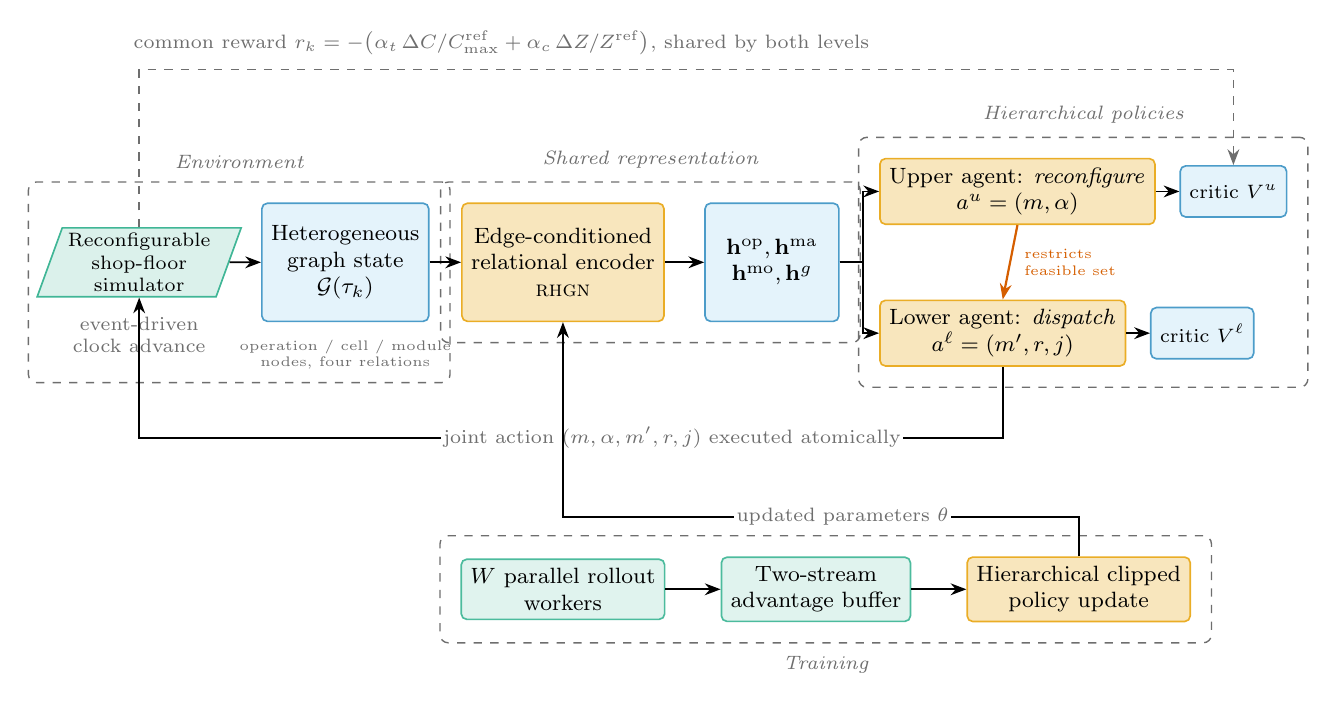
\begin{tikzpicture}[node distance=4mm]

% ============================ environment =============================
\node[datanode, minimum width=20mm] (env) {Reconfigurable\\shop-floor\\simulator};
\node[note, below=1.2mm of env] (envnote) {event-driven\\clock advance};

\node[block, right=4mm of env, minimum width=21mm, minimum height=15mm] (graph)
  {Heterogeneous\\graph state\\$\mathcal{G}(\tau_k)$};
\node[tinynote, below=1.0mm of graph] {operation / cell / module\\nodes, four relations};

% ============================ encoder =================================
\node[keyblock, right=4mm of graph, minimum width=25mm, minimum height=15mm] (enc)
  {Edge-conditioned\\relational encoder\\\textsc{rhgn}};

\node[block, right=5mm of enc, minimum width=17mm, minimum height=15mm] (emb)
  {$\mathbf{h}^{\mathrm{op}},\mathbf{h}^{\mathrm{ma}}$\\$\mathbf{h}^{\mathrm{mo}},\mathbf{h}^{g}$};

% ============================ two agents ==============================
\node[keyblock, right=5mm of emb, yshift=9mm, minimum width=27mm] (upper)
  {Upper agent: \emph{reconfigure}\\$a^{u}=(m,\alpha)$};
\node[keyblock, right=5mm of emb, yshift=-9mm, minimum width=27mm] (lower)
  {Lower agent: \emph{dispatch}\\$a^{\ell}=(m',r,j)$};

\node[block, right=3mm of upper, minimum width=13mm, font=\scriptsize] (cu) {critic $V^{u}$};
\node[block, right=3mm of lower, minimum width=13mm, font=\scriptsize] (cl) {critic $V^{\ell}$};

% main data flow
\draw[arrow] (env) -- (graph);
\draw[arrow] (graph) -- (enc);
\draw[arrow] (enc) -- (emb);
\draw[arrow] (emb.east) -- ++(3mm,0) |- (upper.west);
\draw[arrow] (emb.east) -- ++(3mm,0) |- (lower.west);
\draw[arrow] (upper) -- (cu);
\draw[arrow] (lower) -- (cl);

% conditioning of the lower level on the upper decision
\draw[arrow, draw=oivermilion, line width=0.8pt] (upper.south) -- node[right=0.5mm, font=\tiny, text=oivermilion, align=left] {restricts\\feasible set} (lower.north);

% execution back to the environment: routed below the policy row, above training
\coordinate (retY) at ($(lower.south)+(0,-9mm)$);
\draw[arrow] (lower.south) -- (retY) -| (env.south);
\node[note, whitebg] at ($(retY)+(-42mm,0)$)
  {joint action $(m,\alpha,m',r,j)$ executed atomically};

% Reward feedback. Routed high enough to clear the "Hierarchical policies"
% group label, and delivered to both critics rather than to one of them.
\coordinate (rwY)  at ($(env.north)+(0,20mm)$);
\draw[dasharrow] (env.north) -- (rwY) -| (cu.north);
\node[note, whitebg] at ($(rwY)+(46mm,3.4mm)$)
  {common reward $r_k=-\big(\alpha_t\,\Delta C/\Cmax^{\mathrm{ref}}
   +\alpha_c\,\Delta Z/\Zcost^{\mathrm{ref}}\big)$, shared by both levels};

% ============================ training ================================
\node[block, below=30mm of enc, minimum width=24mm, fill=oigreen!12, draw=oigreen!70]
  (workers) {$W$ parallel rollout\\workers};
\node[block, right=7mm of workers, minimum width=20mm, fill=oigreen!12, draw=oigreen!70]
  (buffer) {Two-stream\\advantage buffer};
\node[keyblock, right=7mm of buffer, minimum width=24mm] (ppo)
  {Hierarchical clipped\\policy update};

\draw[arrow] (workers) -- (buffer);
\draw[arrow] (buffer) -- (ppo);
% updated parameters flow back into the shared encoder and both policy heads
\coordinate (thetaY) at ($(ppo.north)+(0,5mm)$);
\draw[arrow] (ppo.north) -- (thetaY) -| (enc.south);
\node[note, whitebg] at ($(thetaY)+(-30mm,0)$) {updated parameters $\theta$};

\begin{scope}[on background layer]
  \node[group, fit=(env)(envnote)(graph)] (genv) {};
  \node[group, fit=(enc)(emb)] (gnet) {};
  \node[group, fit=(upper)(lower)(cu)(cl)] (gact) {};
  \node[group, fit=(workers)(buffer)(ppo)] (gtrain) {};
\end{scope}
\node[grouplabel, above=0.4mm of genv.north] {Environment};
\node[grouplabel, above=0.4mm of gnet.north] {Shared representation};
\node[grouplabel, above=0.4mm of gact.north] {Hierarchical policies};
\node[grouplabel, below=0.4mm of gtrain.south] {Training};

\end{tikzpicture}
\end{document}
